% !TeX spellcheck = es_AR
\documentclass{beamer}
\usepackage{lmodern}
\usepackage{listings}
\usepackage[T1]{fontenc}
\usepackage[utf8]{inputenc}
\usepackage[spanish]{babel}

\mode<presentation>
{
  \usetheme{Warsaw}
  \setbeamercovered{transparent}
}

\title{Patrones de integración}
\subtitle{Apache Camel y Spring Integration}
\author[Despegar.com]{Pablo Rochás\\ \texttt{pablo.e.rochas@gmail.com}}
\date[Despegar]{Junio 2014}

\begin{document}
\lstloadlanguages{Java,XML}
\begin{frame}
\titlepage
\end{frame}

\begin{frame}{Esquema}
  \tableofcontents
\end{frame}

\section{Introducción}
\subsection{El problema}
\begin{frame}{Integración de sistemas}
¿A qué llamamos integración de sistemas?
\end{frame}

\begin{frame}{El problema}
Problemas de integración al escribir una aplicación
\begin{itemize}[<+->]
\item Distintas aproximaciones por programador
\item Cambios constantes y deuda técnica
\item La experiencia de Ant
\end{itemize}
\end{frame}

\subsection{Soluciones}
\begin{frame}{Soluciones}
\begin{figure}
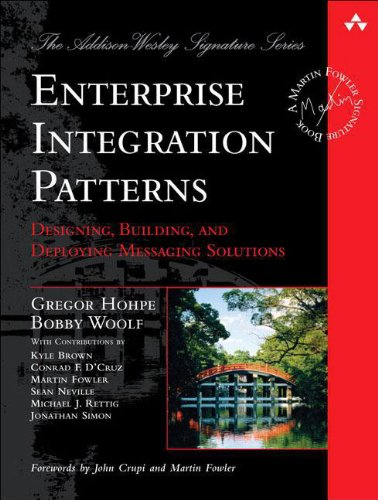
\includegraphics[scale=0.4]{TAPA}
\caption{Editado agosto 2004}
\end{figure}
\end{frame}

\begin{frame}{Soluciones}

\includegraphics[width= 0.9\linewidth]{camel-spring}
\end{frame}

\section{Ejemplos}
\subsection{mailSender}
\begin{frame}[fragile]{Controller}
\lstset{language=Java, basicstyle=\tiny, stringstyle=\bfseries}
\begin{lstlisting}
public class MailSenderController
{
    ...
    private final MessagingTemplate template = new MessagingTemplate();

    @Autowired
    MessageChannel sendChannel;
    ...
    
    private long processRequest(MailRequest req)
    {
      // Arma el mail
      final MimeMessage mimeMessage = mailSender.createMimeMessage();
      ...
      Message<MimeMessage> mailMessage = MessageBuilder.withPayload(mimeMessage)
              .setHeader(MailCheckerHeaders.REQUEST_ID, reqId)
              .setHeader(MailCheckerHeaders.MATCH_TYPE, "sent")
              .build();
      template.send(sendChannel, mailMessage);      
    }
}
\end{lstlisting}
\end{frame}

\begin{frame}[fragile]{XML (1)}
\lstset{language=XML,  basicstyle=\tiny, stringstyle=\bfseries}
\begin{lstlisting}
    <int:channel id="requestChannel" />

    <int:header-enricher input-channel="requestChannel" output-channel="sendChannel">
        <int:header name="mailchecker_match_type" value="sent"/>
    </int:header-enricher>
\end{lstlisting}
\end{frame}

% tapa del libro de EIP
% Se edito en agosto 2004
% los frameworks en _tal_ año
% Diferencias entre las implementaciones:
% - Spring mucho mas cercano al libro
% - Camel mas cómodo y flexible para el programador, se ajusta a su manera de programar
% El ejemplo se desarrolla con spring
% no es la panacea
% preambulo ejemplo: endpoint, channel, message
% ejemplo mail sender
% casos especiales: excepciones, transacciones
% endpoints y/o canales interesantes para destacar (jdbc inbound ch adapter, jpa outbound gateway, etc)
% subscriptions api v3
% wiretap, gateway con java
% conclusiones: no es necesario usar una implementacion, se trata de aprender el lenguaje comun


%\section{Introduction}
%\subsection[Short First Subsection Name]{First Subsection Name}
%\begin{frame}{Make Titles Informative. Use Uppercase Letters.}{Subtitles are optional.}
%\end{frame}
\end{document}